\chapter{Identyfikacja}


\section{Identyfikacja parametrów śmigieł.}

W celu wyznaczenia dynamiki śmigieł helikoptera odpowiedzialnych za ruch odpowiednio względem osi pionowej - Pitch jak i poziomej - Azimuth, przeanalizowano odpowiedzi obiektu na wymuszenie w postaci skoku jednostkowego. Zmiana prędkości obrotowej każdego ze śmigieł, w reakcji na skokową zmianę napięcia zasilania, posłużyła do wyznaczenia parametrów transmitancji. Na bazie przeprowadzonych doświadczeń przyjęto, że każde ze śmigieł jest obiektem inercyjnym pierwszego rzędu w sytuacji gdy sygnałem wejściowym jest napięcie zasilania, a wyjściowym prędkość obrotowa. Do wyznaczenia parametrów tak przyjętego modelu wykorzystano metodę najmniejszych kwadratów. 

\begin{figure}[h!]
	\centering
	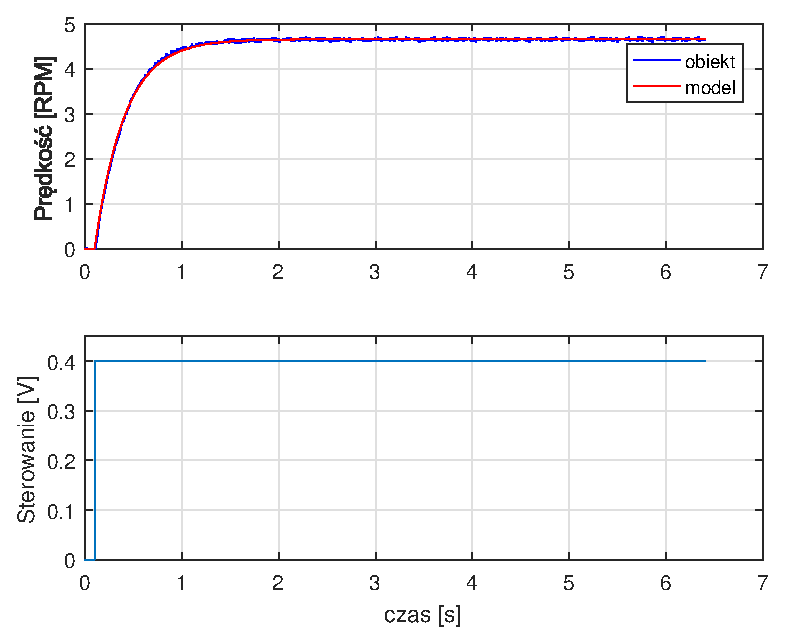
\includegraphics[scale = 1]{fig/Azimuth_iden.eps}
	\caption		
	{Charakterystyka śmigła oś pozioma.}
\end{figure} 
W przypadku osi poziomej model śmigła opisany jest następującą transmitancją:
\begin{equation}\label{key}
G(s) = \frac{K}{Ts + 1} = \frac{11.63}{0.31s + 1}
\end{equation}

\begin{figure}[h!]
	\centering
	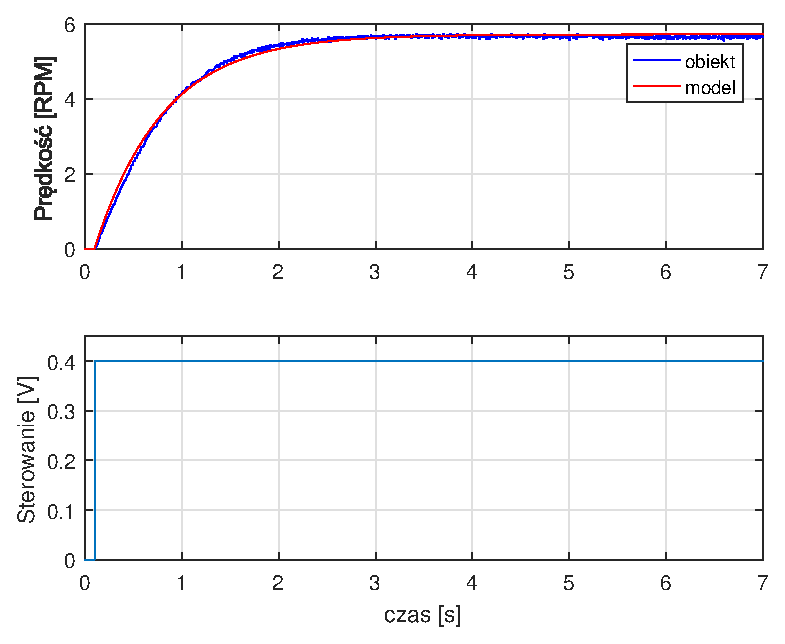
\includegraphics[scale = 1]{fig/Pitch_iden.eps}
	\caption		
	{Charakterystyka śmigła oś pionowa.}
\end{figure} 
Natomiast dla osi pionowej : 
\begin{equation}\label{key}
G(s) = \frac{K}{Ts + 1} = \frac{14.28}{0.71s + 1}
\end{equation}
 
 
\section{Charakterystyka statyczna helikoptera.}

Do wyznaczenia zależności generowanego momentu siły przez śmigło odpowiedzialne za ruch wzdłuż osi pionowej przeprowadzono eksperyment polegający na doczepianiu ciężarków o różnej masie z drugiej strony helikoptera i równoważeniu tak powstałego momentu siły przez odpowiednie dobranie prędkości obrotowej. W tabeli \ref{char_statyczna_tabela} podano otrzymane dane. 
\begin{table}[h]
	\caption{Porównanie poszczególnych regulatorów LQR.}
	\label{char_statyczna_tabela}
	\centering
	
	\begin{tabular}{|c|M{2.5cm}|M{2.5cm}|M{2.5cm}|}
		\hline
		Masa [g]&Prędkość [RPM]&Wsp. PWM [\%]&Moment siły [Nm]\\

		\hline
		0	&	7.1  & 63 & 0.1530\\
		\hline
		15	&  6.3 &  51  & 0.1148\\
		\hline
		30	& 5.2	& 37 &  0.0765\\
		\hline
		45	& 3.75 & 32 &  0.0383\\
		\hline	
		60	& 0	&  0 &  0\\
		\hline
		75	& -5.15	& -33  &   -0.0383\\
		\hline
		90	&	-7.05 & -57 &   -0.0765\\
		\hline
		105	&	-8.7 & -85 & -0.1148\\
		\hline
	\end{tabular}
\end{table}
Na podstawie zależności momentu siły od prędkości wyznaczono wielomian aproksymujący rzędu trzeciego opisanego zależnością : 
\begin{equation}\label{key}
M(v) = -0.0002v^3 -0.0009 v^2  - 0.0061v + 0.1571
\end{equation}

\begin{figure}[h!]
	\centering
	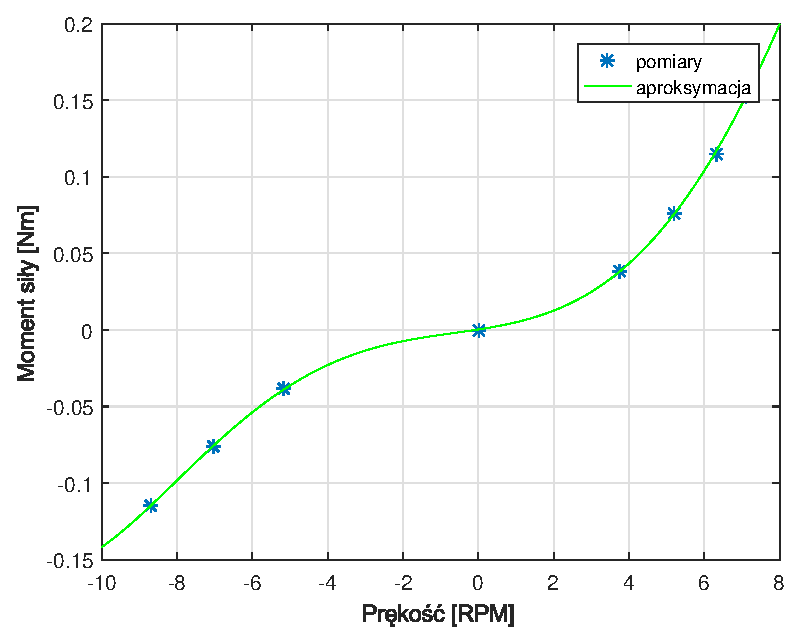
\includegraphics[scale = 1]{fig/char_statyczna.eps}
	\caption		
	{Charakterystyka statyczna śmigła oś pionowa.}
\end{figure}

Chcąc znalezć zależność pomiędzy wartościami odczytywanymi z tachopradnicy a rzeczywistą prędkością obrotową śmigła sporządzono charakterystykę statyczną napięcia na tachoprądnicy od jej sygnału wyjściowego. Z racji na liniową zależność, otrzymane dane pomiarowe aproksymowano funkcją liniową w postaci:
\begin{equation}\label{key}
U(x) = 0.164 \cdot x + 0.0019
\end{equation}
Dane pomiarowe z wyznaczoną funkcją aproksymującą zaprezentowane są na rysunku \ref{skal_pred}.
\begin{figure}[h!]
	\centering
	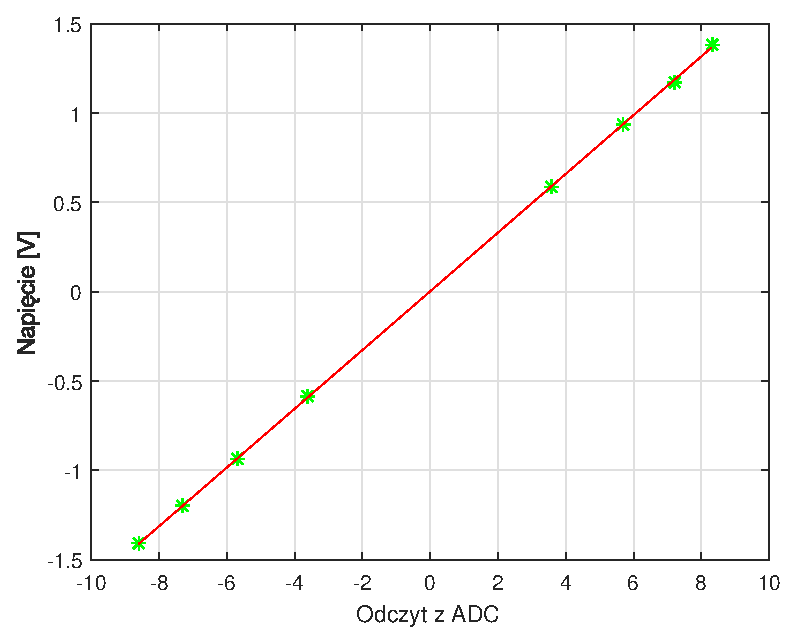
\includegraphics[scale = 1]{fig/skal_predkosci.eps}
	\caption		
	{Skalowanie prędkości obrotowej śmigła.}
	\label{skal_pred}
\end{figure}
Finalnie otrzymano następującą zależność na prędkość obrotową wirnika: 
\begin{equation}\label{key}
RPM = (0.164 \cdot x + 0.0019 ) * \frac{1}{0.52}
\end{equation}
\begin{figure}[h!]
	\centering
	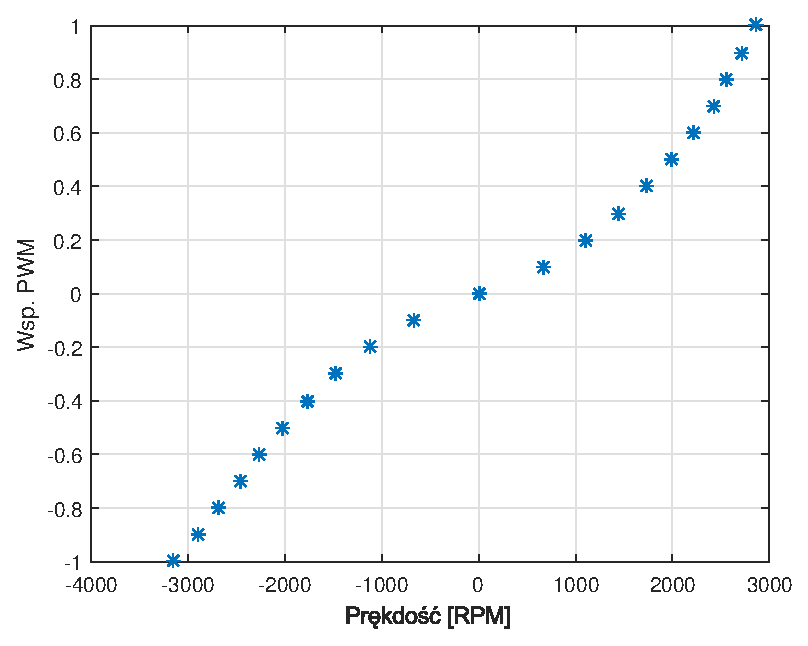
\includegraphics[scale = 1]{fig/PWM_predkosci.eps}
	\caption		
	{Zależność pomiędzy współczynnikiem wypełnienia PWM i prędkością obrotową.}
	\label{PWM_pred}
\end{figure}

\section{Moment bezwładności}
\subsection{Oś "pitch"}
W celu wyznaczenia momentu bezwładności helikoptera względem punktu podporu przyjęto oscylacyjny model obiektu. W celu wyznaczenia parametrów opisujących dynamikę, przeprowadzono eksperyment polegający na rejestracji gasnących oscylacji układu po wychyleniu go z położenia równowagi o zadany kąt. Następnie na postawie zarejestrowanych danych i funkcji  \textit{lsqnonlin} dobrano parametry równania \ref{tr_bezwl} minimalizując kwadrat różnicy pomiędzy odpowiedzią obiektu i modelu. Na rysunku \ref{rys_bezwl} przedstawiono porównanie odpowiedzi obiektu i modelu. 
\begin{equation}\label{tr_bezwl}
Ku(t) = \frac{d^2\alpha(t) }{dt^2} + 2\xi \cdot \omega \cdot \frac{d\alpha(t) }{dt} + \alpha(t) \cdot \omega^2
\end{equation}
\newpage
Na drodze optymalizacji otrzymano następujące wartości parametrów:\\
$
K = 1 \\
\xi = 0.013 \\
\omega = 2.2247\\
$

Moment bezwładności helikoptera wyznaczono z zależności pomiędzy momentem bezwładności wahadła fizycznego, a okresem drgań równanie \ref{zal_bezw}.\\
 \begin{equation}\label{zal_bezw}
 J = (\frac{T}{2\pi})^2
 \end{equation}
 gdzie: \\
 $J$ - moment bezwładności\\
 $T = \frac{2\pi}{\omega}$ - okres drgań własnych\\\\
\begin{figure}[h!]
	\centering
	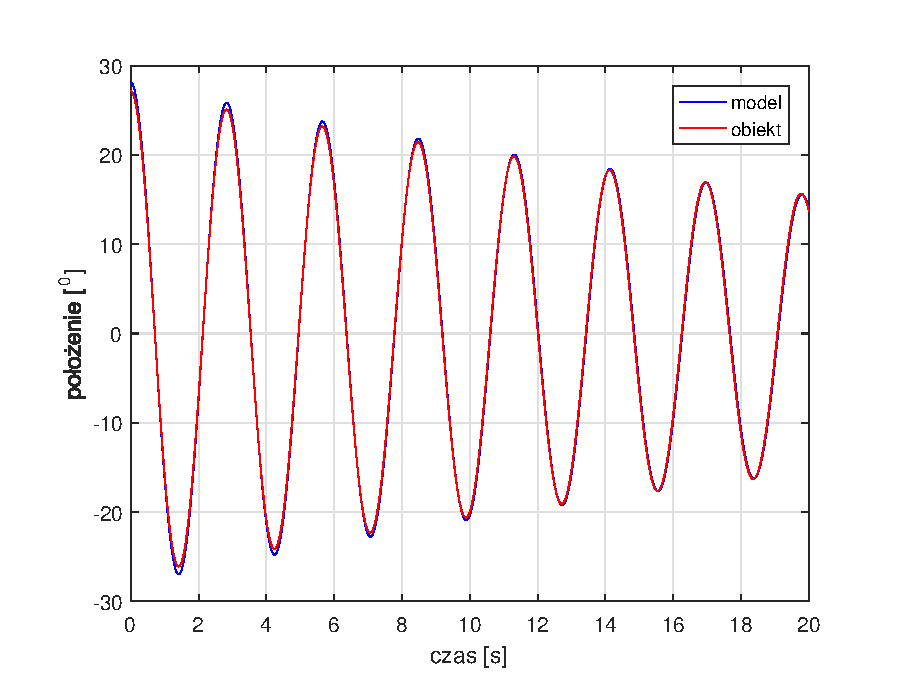
\includegraphics[scale = 1]{fig/bezwladnosc.eps}
	\caption		
	{Porównanie odpowiedzi obiektu i modelu.}
	\label{rys_bezwl}
\end{figure}
W efekcie końcowym wartości momentu bezwładności wynosi $J = 0.202 \ kg \cdot m^2.$